\subsection{Hyperledger}

\textit{Author: Julian} \\
In Hyperledger Burrow the throughput was measured using the $Throughput_{alt}$ method mentioned in 2.1.
In Table \ref{table:4} the minimum, maximum and average time of a transaction is visualized. For 10 up to 1000 transactions
the minimum and average time of one transaction is below 1 second. The maximum time for 1000 transactions is at around 25
secounds and it increases drastically to around 1000 seconds, if the transactions increase to 10000.

\begin{table}[!h]
\centering
\begin{tabular}{l|l|l|l|}
\hline
\multicolumn{1}{|l|}{\textbf{tx}} & \textbf{Min {[}s{]}} & \textbf{Max {[}s{]}} & \textbf{Avg {[}s{]}} \\ \hline
\multicolumn{1}{|l|}{\textit{10}} & \textit{0.436} & \textit{0.632} & \textit{0.530} \\ \hline
\multicolumn{1}{|l|}{\textit{100}} & \textit{0.379} & \textit{0.644} & \textit{0.475} \\ \hline
\multicolumn{1}{|l|}{\textit{1000}} & \textit{0.387} & \textit{25.557} & \textit{0.572} \\ \hline
\multicolumn{1}{|l|}{\textit{10000}} & \textit{0.359} & \textit{999.583} & \textit{3.457} \\ \hline 
\end{tabular}
\caption{Burrow: Min, Avg and Max execution time of a transaction}
\label{table:4}
\end{table}

The throughput for the test with 10 transactions is displayed in Fig. \ref{fig:burrowtxs} the upper left graph shows a more or less
stable curve with only few a ups and downs and not much variation. The result for 100 (Fig. \ref{fig:burrowtxs} upper right)
transactions has a similar outcome. Starting the benchmark with 1000 (Fig. \ref{fig:burrowtxs} lower left) or even 10000
(Fig. \ref{fig:burrowtxs} lower right) transactions, the variance of some of these measurements is extremly high. In
the last test, the effect even intensifies with more time passing. \\[5mm]

\begin{minipage}{\linewidth}
    \makebox[\linewidth]{
    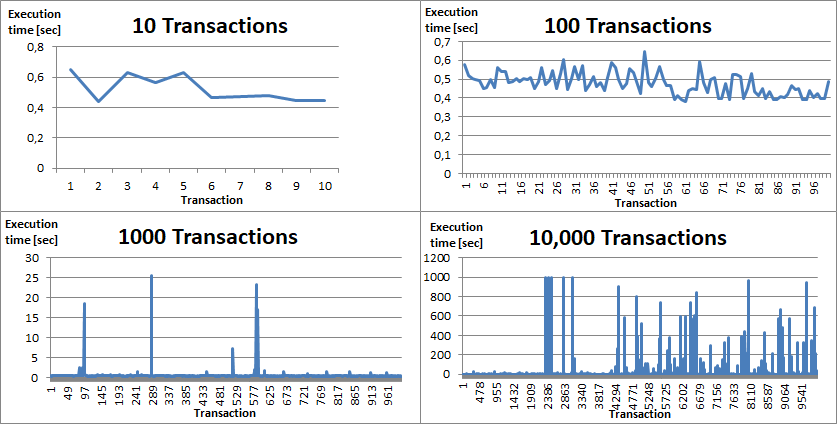
\includegraphics[width=1.00\textwidth]{img/HyperAllInOne.png}}
   \captionof{figure}{Burrow: Transactions and their execution time}\label{fig:burrowtxs}
\end{minipage}

The increase in the time needed to execute one transaction with a higher total number of transactions sent is part of the
limitations of the used EC2 instance. The thread pool used to send multiple transactions at once were to many for the engine
to handle and in the end the node ran out of free memory. This effect could be weakened by decreasing the thread pool size
but would also result in a higher total execution time. A test was done with 1000 transaction and a pool size of 10 and 150.
Where the total execution time of the first one was around 20 minutes, the second one was below 4 minutes. \\[5mm]

The calculated throughput for these four benchmarks is shown in Fig. \ref{fig:burrowthroughput}. It is apparent, that the throughput
is decreasing the more transactions are sent. Where for the test with only 10 transactions it would sum up to above 80 transactions per second.
The test with 10000 transactions resulted in less than 30 transactions per second.

\begin{minipage}{\linewidth}
    \makebox[\linewidth]{
    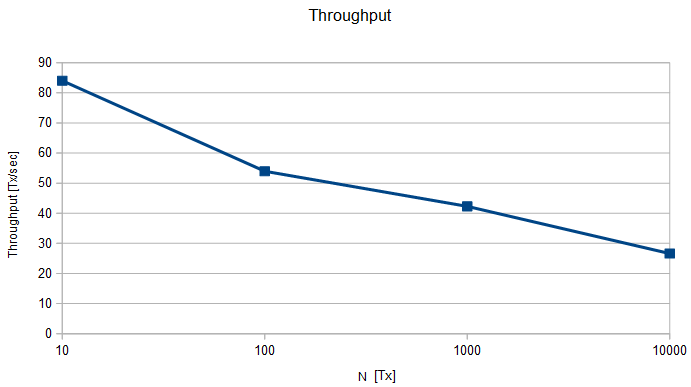
\includegraphics[width=0.75\textwidth]{img/Hyperledger.png}}
   \captionof{figure}{Burrow: Throughput}\label{fig:burrowthroughput}
\end{minipage}
